\documentclass{llncs}

\usepackage{amsmath}
\usepackage{../Utils}
\usepackage{pdfsync}

\newcommand{\sds}[1]{{\textcolor{blue}\small\marginpar{}}}
\renewcommand{\emph}[1]{{\em #1}}
\begin{document}


\title{Describing Layered Architectures in Haskell}
\titlerunning{Describing Layered Architectures in Haskell}

\author{Martijn M. Schrage\inst{1} \and S. Doaitse Swierstra\inst{2}}
\institute{Oblomov Systems, Utrecht, \email{martijn@oblomov.biz}
\and Department of Computer Science, Utrecht University, \email{doaitse@cs.uu.nl}}

\maketitle

\begin{abstract}
We define a domain specific embedded language in Haskell for describing
layered software architectures which maintain bidirectional dependencies. By using a typed programming
language to describe the architecture, the correct composition of its components
is guaranteed by the type checker of the language. Because, contrary to the situation with typical Architecture Description Languages, the
description is part of the implementation they are guaranteed to comply with each other. Finally we show how to use the Haskell class system to define a more general form of composition.
\end{abstract}

% \category{D.2.11} {Software Engineering}
%                   {Software Architectures}
%                   [Languages (e.g., description, interconnection, definition)]

% \terms
% Domain-specific languages, Architecture

% \keywords
% Haskell, Layered architectures, Architecture descriptions, Type-level programming
\section{Introduction}\label{sect:introduction}

In a survey~\cite{medvidovic00ADLs} of architecture description languages (ADL), three essential components of an architecture description are identified: a description of the (interface of the) \emph{components}, a description of the \emph{connectors}, and a description of the architectural \emph{configuration}. The claim is that the focus on conceptual architectures and the explicit treatment of connectors as first-class entities differentiate architecture description languages from, amongst others, programming languages. We claim the opposite, and show how a \emph{collection of Haskell functions} can be combined into a component, how the \emph{parameter and result types} of these functions represent the connectors, and how configurations can be described by Haskell expressions built with the use of \emph{architectural combinators}. We substantiate our claim by developing a set of Haskell combinators for describing architectures of layered systems. Although designed with a layered editor in mind, we claim this approach to be applicable to many kinds of architectures. The combinators have been successfully used in the implementation of the generic editor Proxima~\cite{Schrage04Proxima}.

Describing an architecture in an real programming language not only makes it possible to describe the interfaces of the components of the system, and how they are to be composed, but also enables us to smoothly extend this high-level description into a real implementation, without having to maintain several, probably conflicting views on our system. Because the architecture description in Haskell is a program in itself, the system can be instantiated by providing implementations for each of the components. By embedding our architecture description language~\cite{hudak98DSLs} inside a general purpose programming language,we can reuse the syntax, semantics, implementation code, software tools, as well as the look-and-feel. Besides this we can easily combine the language with other embedded languages in the same program.

In Section \ref{sect:layerInHaskell} we show how to describe layers composed of functions, and how to combine layers into composite layers. In Section \ref{sect:lib} we develop combinators which help in this process. In Section \ref{sect:typeClass} we show how to use the Haskell class system to generalise over the described interfaces. In Section \ref{sect:proxima} we show an actual use of the combinators, and in the last section we conclude.
\sds{add summary}
% In this paper we give three implementation models for layered architectures. First, in Section~\ref{sect:simpleEditor}, we introduce a simplified layered editor architecture and, in section~\ref{sect:layerInHaskell}, explore how its main components can be modeled in Haskell. Then we proceed to connect the components. In Section~\ref{sect:simple} the connection is straightforward, with little abstraction. This is used as a basis in Section~\ref{sect:ncp} as a base to develop a more abstract combinator implementation that uses nested pairs. In Section~\ref{sect:hidden}, we present another set of combinators, which employ a form of state hiding to improve on the previous set. Section~\ref{sect:lib} develops a small generic library for building the architecture-specific combinators of Section~\ref{sect:hidden}. The combinators from this section require two minimal function definitions for instantiating a specific architecture. In Section~\ref{sect:typeClass}, we exploit the type system to automatically provide these definitions, based solely on the types of the layer interface. Section~\ref{sect:proxima} shows how the architecture combinators are used to describe (and implement) the architecture of the Proxima editor. And, finally, Section~\ref{sect:conclusions} discusses future work and concludes.
			
			
			
\renewcommand{\textfraction}{0} 
\begin{figure}{t}
\includegraphics[width=\columnwidth]{images/LayersDataFlow}
\caption{Data flow in and between layers.} \label{explicit} 
\end{figure}													\section{Layered Architectures}\label{sect:layerInHaskell}

The architecture description combinators in this paper have been designed for the generic presentation-oriented structure editor Proxima, which supports editing both on the document structure as well as on its presentation, Proxima is organised as a sequence of layers (each taking care of some aspect of converting an abstract document into a screen bitmap), in which  each layer maintains its own local state. Examples of such state are white space, visibility toggles, alignment information, formatting directives, and unfolding status. 

%Because of the complexity of the actual Proxima architecture, we introduce a simple layered architecture for a presentation-oriented editor to explain the architecture description methods. Although the architecture is simple, it contains the essential features of the Proxima architecture. 
In Figure \ref{explicit} we sketch the flow of data in a typical Proxima implementation. On the top left we see the input of type \p{doc}, which is mapped by successive of \p{present} functions onto a presentation \p{pres3}. This presentation is shown on the screen, after which the user inputs a gesture \p{gest3}, which is mapped back by a sequence of \p{interpret} functions onto an updated document \p{update}. At each level we see state information (for the \p{interpret} function typically also containing a \p{map} to keep track of where things end up on the screen), being passed on horizontally. The states at each level resulting from the \p{interpret} functions are used in the next editing cycle, and so are fed back at the left of the picture.
	
A layer can be seen as an architectural component, something typically represented as a box with connectors in a graphical architecture description language. We will compose the box out of functions, and the arguments and results of these function will constitute the connectors. In our editor example a layer first ``communicates'' by accepting a document to be presented, internally maps this documents onto something which is presented at an output port connected to the lower layer while updating its internal state, next accepts a gesture from the lower layer, and presents an updated document to the layer above, possibly again updating its internal state. So besides having the connector types following from the types of the arguments and results of the internal functions, we also have a ``protocol'', i.e. an order in which the communication takes place at the connectors and in which direction. 
If we capture this protocol of a Proxima layer in a type we get (forced to use a \p{newtype} since Haskell does not allow recursive types):

\begin{small}
\begin{verbatim}
newtype Layer doc pres gest upd = Layer ( doc -> ( pres, ( gest -> ( upd , 
        Layer doc pres gest upd))))
\end{verbatim}
\end{small}

\noindent The important part is the last part of the first line, in which the communication types are listed: \p{doc} and \p{gest} correspond to communication at an input port, and \p{pres} and \p{upd} communication at an output port. The type parameters indicate what kind of information is communicated. Note furthermore that the type of the internal state, which is irrelevant from an architectural point of view, is invisible from this type.

We define a combinator \p{combine}, which combines a higher layer and a lower layer into a single composed layer: an architectural composition. Its type is:

\begin{small}
\begin{verbatim}
combine :: Layer high med emed ehigh -> Layer med low elow emed -> 
           Layer high low elow ehigh
\end{verbatim}
\end{small}

The reason for the order of the type variables is that for each pair of variables, the first type is an argument type and the second type  a result type. Hence, the first step in the combined layer is a function \p{high -> low}, which is the composition of a function \p{high -> med} in the higher layer and a function \p{med -> low} in the lower. On the other hand, the second step goes upward.  Thus, the function \p{elow -> ehigh} in the combined layer is the reverse composition of functions \p{elow -> emed} and \p{emed -> ehigh} in the higher and lower layers 
The implementation of combine is a straightforward plumbing --completely controlled by the types-- to get the parameters at the right places. The direction of the vertical parameters is encoded in the definition of \p{combine}. Note that in the code below \p{high} and \p{elow} again correspond to communication at an input port, and \p{low} and \p{ehigh} to communication at an output port.

\begin{small}
\begin{verbatim}
combine (Layer upr) (Layer lwr) = Layer $ exec upr lwr
 where exec upr lwr =  \high -> let (med, uprIntr) = upr high 
                                    (low, lwrIntr) = lwr med
                                in  (low, 
                       \elow -> let (emed, lwr)  = lwrIntr elow 
                                    (ehigh, upr) = uprIntr emed
                                in  (ehigh, 
                       exec upr lwr)
\end{verbatim}%$
\end{small}

The edit loop of the simple editor uses a combined component by following its presented \p{Layer} protocol:

\begin{small}
\begin{verbatim}
editLoop :: (GetGesture gest, ShowRendering pres, Updateble update doc) =>
            Layer doc pres gest update -> doc -> IO ()
editLoop (Layer presentStep) doc = 
 do { let (pres , interpretStep) = presentStep doc    
    ; showRendering pres
    ; gesture <- getGesture    
    ; let (update, presentStep') = interpretStep gesture      
    ; editLoop presentStep' (updateDocument update doc)
    }
\end{verbatim}
\end{small}



\section{Developing a library for architecture descriptions} \label{sect:lib}

In the previous section we have hard-coded the interface (protocol) of a layer in the \p{combine} combinator: information was flowing down and up in an alternating way. The \p{combine} combinator from the previous section is just one case of a layered architecture: a layer with two layer functions and hence two {\em step}s, where a {\em step} is an alternation of in input and an output communication.

Even though the code for \p{combine} was straightforward, some code is duplicated, and small errors are easily made. Therefore, instead of a guideline on how to write \p{combine} by hand, we develop a small library of meta combinators for constructing such \p{combine} functions for any sequence of steps. A further  advantage of having  a meta-combinator library is that instead of explicitly encoding the direction for each of the steps in the \p{combine} function, we can use the name of the meta combinator to reflect the direction in which the data flows. 


\subsection{Type definitions} \label{subsecttypedef}

The \p{Layer} type poses a problem if we want to construct a library for building \p{lift} and \p{combine} functions, since somehow its constructors need to be added to and removed by the combinators, and furthermore the number of type parameters is fixed. Therefore, we introduce a compositional representation of a layer type that makes use of simple types defined in the library.

If we inspect the \p{Layer} type we see it is made up of two steps of the form \p{vArg -> (vRes, ...)}, hence we capture the concept of a single step: 

\begin{small}
\begin{verbatim}
newtype Step a b ns = Step (a -> (b, ns))
\end{verbatim}
\end{small}

\bc
Using GADT's one might even make the fact that a step function should be seen as function by using the following formulation:

\begin{small}
\begin{verbatim}
newtype Step :: * -> * -> * where Step :: (a -> (b, ns)) -> Step (a -> b) ns
\end{verbatim}
\end{small}
\ec

In order to compose steps, we define an infix, right-associative, type constructor \p{(:.:)} a, and a type to represent the absence of further steps:.

\begin{small}
\begin{verbatim}
infixr :.:
newtype (:.:) f g ns  = Comp (f (g ns))
newtype NilStep t = NilStep t
\end{verbatim}
\end{small}

The type \p{Doc -> (Pres, Gest -> (Upd, next))} is now encoded as
\p{(Step Doc Pres :.: Step Gest Upd :.: NilStep) next}. To encode the feedback loop, we introduce a fixed-point type \p{Box}, which builds an architectural box:

\begin{small}
\begin{verbatim}
newtype Box f = Box (f (Box f))
\end{verbatim}
\end{small}

With these type combinators, we can now express \p{Layer} in a compositional way:

\begin{small}
\begin{verbatim}
type Layer d p g u = Box (Step d p :.: Step p u :.: NilStep)
\end{verbatim}
\end{small}

Because \p{Step}, \p{NilStep}, and \p{:.:}  appear partially parametrized in the layer type, and \p{Box} is recursive, all three types need to be introduced using \p{newtype} definitions. Hence, instead of having a single \p{Layer} constructor, \p{combine} will be littered with constructors; the combinators we will derive in the next subsections take care of adding and removing these constructors.

The reason why we have an explicit \p{NilStep} with yet another constructor is that it causes the number of occurrences (\p{:.:}) to be the same as the number of steps, which will facilitate the removal of \p{Comp} constructors.
\subsection{Derivation for \p{liftStep}}\label{subsect:liftDerivation}

The first thing to so now it to define a function \p{liftStep} which takes a single layer function, and converts it into a primitive box:

\begin{small} % lift2
\begin{verbatim}
liftStep f next horArgs = Comp . Step $ mapSnd next .(f horArgs)
lNilStep next hRes = NilStep $ next hRes
\end{verbatim}%$
\end{small}

Here we see why composition is right associative, since each step has both a\p{Comp} constructor which as its left operand assumes a \p{Step} constructor. 
%If composition were left-associative, the \p{Comp} constructors would end up between the \p{Box} and \p{Step} constructors, and it would be harder to capture the pattern.


Regardless the number of steps, there will only be one \p{Box} constructor (in contrast to the number of \p{Comp} and \p{Step} constructors, which are equal to the number of steps). Hence, we can define a function \p{lfix} to add this constructor. The function \p{lfix} also closes the steps with a \p{lNilStep}. 

\begin{small}% lift5
\begin{verbatim}
lfix f = fix f' where f' n = Box . (f . lNilStep) n
         where fix a = let fixa = a fixa in  fixa
\end{verbatim}
\end{small}

Now suppose we have a pair of layer functions be want to combine into a single layer, then we can write:
\begin{small}% lift5
\begin{verbatim}
data   Simple state1 state2 doc pres gest upd 
     = Simple (state1 -> doc  -> (pres, state2))
              (state2 -> gest -> (upd, state1))
\end{verbatim}
\end{small}

Using \p{liftStep} we can now easily combine the two functions:

\begin{small} % lift
\begin{verbatim}
lift :: Simple state1 state2 doc pres gest upd ->
        state1 -> Layer doc pres gest upd
lift (Simple present interpret)= lfix $ 
                                 liftStep present . liftStep interpret
\end{verbatim}%$
\end{small}

\bc
For an $n$-step layer, the definition of \p{lift} has $n$ local step functions, each  containing a reference to the next. \bc \note{mention that the last one refers to the first?} \ec For such a layer, we can perform exactly the same steps as for the 2-step \p{lift}. The resulting \p{lift} contains a composition of $n$ \p{liftStep} applications. If we denote the step type constructors by \p{Step$_i$} and the layer functions by \p{layerFn$_i$}, we get:

\begin{small}
\begin{tabbing}
{\tt lift layer = } \= {\tt lfix \$ liftStep (layerFn$_1$ layer)} \\
                    \>       \dots \\
                    \> {\tt .~~~~~~liftStep (layerFn$_n$ layer)}\\
\end{tabbing}%$
\end{small}
\ec
\subsection{Derivation for \p{combine}} \label{subsubsectcombine}


The derivation of the meta combinators for \p{combine} is largely similar to the derivation for \p{lift}. We start with a definition of \p{combine} for a two-step layer, adapt it to the new \p{Layer} type and rename several variables:
\sds{have we mentioned this?}
\begin{small} % combine0
\begin{verbatim}
combine (Box upr) (Box lw)r = step1 upr lwr
 where step1 (Comp (Step upr)) (Comp (Step lwr)) = 
         Box. Comp . Step $ \high -> let (med, uprIntr) = upr high
                                         (low, lwrIntr) = lwr med
                                     in  (low, step2 uprIntr lwrIntr)
       step2 (Comp (Step upr)) (Comp (Step lwr)) = 
         Comp . Step $ \low -> let (med, lwrPres) = lwr low
                                   (high, uprPres) = upr med
                               in  (high, cNilStep uprPres lwrPres)
       cNilStep (NilStep u) (NilStep l) = NilStep $ step1 u l 
\end{verbatim}%$
\end{small}

The explicit mutual recursion in the local functions is removed by passing the next step as a parameter, and rewriting the whole function as a fixed point. The \p{cNilStep} becomes a top-level function.

\begin{small} %combine2
\begin{verbatim}
combine (Box upr) (Box lwr) = fix (step1 . step2 . cNilStep) upr lwr
 where step1 next (Comp (Step upr)) 
                  (Comp (Step lwr)) = 
         Box. Comp . Step $ 
         \high -> let (med, uprIntr) = upr high
                      (low, lwrIntr) = lwr med
                  in  (low, next uprIntr lwrIntr)
       step2 next (Comp (Step upr)) (Comp ( Step lwr)) = 
         Comp . Step $
         \low -> let (med, lwrPres) = lwr low
                     (high, uprPres) = upr med
                 in  (high, next uprPres lwrPres)

cNilStep next (NilStep u) (NilStep l) = 
  NilStep $ next u l
\end{verbatim}%$
\end{small}

Without the explicit recursive calls, we can capture the vertical data flow patterns with two functions \p{combineStepDown} and \p{combineStepUp}:

\begin{small} 
\begin{verbatim}
combineStepDown :: (f x -> g y -> h ns) -> 
                   (Step a b :.: f) x -> 
                   (Step b c :.: g) y -> 
                   (Step a c :.: h) ns
combineStepDown next (Comp (Step upper)) 
                     (Comp (Step lower)) = Comp . Step $
  \h -> let (m ,upperf) = upper h
            (l, lowerf) = lower m
        in  (l, next upperf lowerf)   

combineStepUp :: (f x -> g y -> h ns) ->
                 (Step b c :.: f) x ->
                 (Step a b :.: g) y ->
                 (Step a c :.: h) ns
combineStepUp next (Comp (Step upper)) 
                   (Comp (Step lower)) = Comp . Step $ 
  \l -> let (m, lowerf) = lower l
            (h, upperf) = upper m
        in  (h, next upperf lowerf)   
\end{verbatim}%$
\end{small}

Now we can define a function \p{cfix} that pattern matches on the arguments and adds a \p{Box} to the result. Similar to \p{lfix}, it also adds the \p{cNilStep}.

\begin{small}
\begin{verbatim}
cfix f = fix f' where f' n (Box u) (Box l) = Box $ (f . cNilStep) n u l
\end{verbatim}%$
\end{small}

The final version of \p{combine} now reads:

\begin{small}%combine
\begin{verbatim}
combine :: Layer high med emed ehigh -> Layer med low elow emed -> 
           Layer high low elow ehigh
combine = cfix (combineStepDown . combineStepUp)
\end{verbatim}
\end{small}


Similar to \p{liftStep}, \p{combineStepDown} and \p{combineStepUp} do not depend on the number of steps. Hence, they can be used to construct \p{combine} for layers with an arbitrary number of layer functions.

\bc
The editing loop changes at a few places, in order to remove the extra introduced constructors, which become visible at the outside of the constructed component, which we are going to use now. Just as \p{combine} and \p{liftStep} have to be aware of these constructors, and so has \p{editLoop}:

\begin{small}
\begin{verbatim}
unStep (Comp (Step step)) = step
unNil  (NilStep step)      = step

editLoop (Box presentStep) doc = 
 do { let (pres , interpretStep) = 
            unStep presentStep $ doc   
    ; showRendering pres
    ; gesture <- getGesture    
    ; let (update, presentStep') = unStep interpretStep $ gesture    
    ; let doc' = updateDocument update doc
    ; editLoop (unNil presentStep') doc'
    }
\end{verbatim}%$
\end{small}
\ec
\subsection{Adding a monad}


The final modification we make to the library is to add a monad, in order to allow layer functions to perform IO operations. The type \p{LayerFn} is extended with an extra type variable \p{m} for the monad.

\begin{small}
\begin{verbatim}
type LayerFn m horArgs vertArg horRess vertRes 
  = horArgs -> vertArg -> m (vertRes, horRess)
\end{verbatim}
\end{small}

Without further comment we redefine our types to account for the monadic result:

\begin{small}
\begin{verbatim}
newtype Step a b m ns = Step (a -> m (b, ns))
newtype (:.:) f g m ns  = Comp (f m (g m ns))
newtype NilStep m t = NilStep t
\end{verbatim}
\end{small}

\noindent
For the fixed point, we introduce a type synonym \p{BoxM}, which passes the monad to its type-function argument, and applies \p{Box} to the result.

\begin{small}
\begin{verbatim}
type BoxM m f = Box (f m)
\end{verbatim}
\end{small}

The monadic version of the other code is largely similar to the non-monadic version. Basically, each let expression of the form\\

\noindent
\p{\small let x$_1$ = $exp_1$; \dots ; x$_n$ = $exp_n$ in ($hRes$,$vRes$)}\\

is replaced by a monadic statement\\

\noindent
\p{\small do \{ x$_1$ <- $exp_1$; \dots ; x$_n$ <- $exp_n$; return ($hRes$,$vRes$) \}}\\

Furthermore, the type signatures for the pairs of horizontal and vertical results \p{($hRes$, $vRes$)} become \p{m ($hRes$, $vRes$)}. Because of the similarity between the two libraries, we only show the monadic \p{liftStep}:

\begin{small}
\begin{verbatim}
liftStep :: (hArg -> vArg-> m (vRes, hRes)) -> 
            (hRes -> ns) -> hArg -> Step vArg vRes ns
liftStep f next horArgs = Step $ 
  \vArg -> do { (vertRes, horRes) <- f horArgs vArg
              ; return (vertRes, next horRes)
              }
\end{verbatim}
\end{small}%$

The functions \p{lfix}, \p{lcomp}, \p{cfix}, and \p{ccomp} are independent of the monad and are the same for both versions of the library. The full code of the library can be found in a technical report, which contains a longer account of the design steps given here~\cite{UUCS2008045}

In order to describe and implement an architecture, we need to provide a \p{Layer} type, and definitions of \p{lift} and \p{combine}. We give a general description of these definitions.
The general case that we consider is a layer with $n$ layer functions. The record type \p{TheLayer m h$_1$ \dots ~h$_m$ a$_1$ r$_1$ a$_2$ r$_2$ \dots ~a$_n$ r$_n$} contains the layer functions. The variable \p{m} is the monad, variables \p{h$_i$} are the types that appear in the horizontal parameters of the layer, and the \p{a$_i$} and \p{r$_i$} are the types of the vertical arguments and results. 

Because the types of the horizontal parameters are not necessarily single \p{h$_i$} variables, but tuples of these variables, we denote the horizontal parameters by $horArgs_i$ and $horRess_i$. As an example, consider the type \p{Simple}. Its horizontal  type variables are \p{map} and \p{state}, but the types of the horizontal parameters are \p{state} and \p{(map, state)}. In general, the definition of \p{TheLayer} has this form:

\begin{small}
\begin{tabbing}
{\tt da}\={\tt ta}\\
\> {\tt Th}\={\tt eLayer~m h$_1$ \dots ~h$_m$ a$_1$ r$_1$ a$_2$ r$_2$ \dots ~a$_n$ r$_n$ = }\\
\> \> {\tt TheLayer~}\={\tt \{~LayerFn$_1$}\verb| :: |{\tt LayerFn~m~}\= {\tt $horArgs_1$ a$_1$}\\
\> \>                \>                                             \> {\tt $horArgs_2$ r$_1$}\\
\>\>\> {\tt , LayerFn$_2$}\verb| :: |{\tt LayerFn~m~}\={\tt $horArgs_2$ a$_2$}\\
\> \>                \>                            \>{\tt $horArgs_3$ r$_2$ \}}\\
\>\>\> {\tt \dots }\\
\>\>\> {\tt , LayerFn$_n$}\verb| :: |{\tt LayerFn~m~}\={\tt $horArgs_{n}$ a$_n$}\\
\> \>                \>                            \>{\tt $horArgs_1$ r$_n$ \}}\\
\end{tabbing}
\end{small}

We assume the layer is normalized, meaning that $horArgs_{1} = horRess_n$ and 
$horArgs_{i+1} = horRess_i$. If the layer is not normalized, a simple wrapper function can be defined to convert the layer to a normalized layer (see Section~\ref{sect:layerInHaskell}). 

For a layer record as defined above, the type definition for the \p{Layer} type used by the combinators is:

\begin{small}
\begin{tabbing}
{\tt ty}\={\tt pe Layer m a$_1$ r$_1$ a$_2$ r$_2$ \dots ~a$_n$ r$_n$ =}\\
        \>{\tt BoxM m (Step a$_1$ r$_1$ :.: a$_2$ r$_2$ :.: \dots ~:.: Step a$_n$ r$_n$)}
\end{tabbing}
\end{small}

The definitions of \p{lift} and \p{combine} are straightforward. For \p{lift}, we need to apply \p{liftStep} to each of the layer functions, compose the steps with \p{lcomp}, and apply \p{lfix} to the composition. 

\begin{small}
\begin{tabbing}
{\tt lift}\verb| :: |\={\tt Monad m =>}\\
                     \>{\tt TheLayer m h$_1$ \dots ~h$_m$ a$_1$ r$_1$ \dots ~a$_n$ r$_n$ -> Layer m a$_1$ r$_1$ \dots ~a$_n$ r$_n$}\\
{\tt li}\={\tt ft t}\={\tt heLayer = }\\
\>{\tt lfix \$ liftStep (LayerFn$_1$ theLayer)}\\
\>\verb|     . lift|{\tt Step (LayerFn$_2$ theLayer)}\\
\>{\tt ~~~~~\dots}\\ 
\>\verb|     . lift|{\tt Step (LayerFn$_n$ theLayer)}
\end{tabbing}
\end{small}%$


The \p{combine} combinator consists of $n$ \p{combineStepUp$/$Down} meta combinators, composed with \p{ccomp}, after which \p{cfix} is applied. The direction of the vertical data flow determines the choice between \p{combineStepUp} and \p{combineStepDown} for each step.  The exact type of \p{combine} depends on the direction of the meta combinators and is explained below. 

\begin{small}
\begin{tabbing}
{\tt combine}\verb| :: |\={\tt Monad m => Layer m \dots}\verb| -> |{\tt Layer m \dots}\verb| -> |{\tt Layer m \dots }\\
{\tt co}\={\tt mbine}\={\tt ~=  cfix \$ combineStepUp$/$Down \dots \ \ combineStepUp$/$Down}
\end{tabbing}%$
\end{small}

The type of \p{combine} depends on the direction of the vertical data flow in the layer. Consider the $i$-th pair of  type variables in \p{Layer a$_1$ r$_1$ \dots~a$_n$ r$_n$}. Variable \p{a$_i$} represents the vertical argument of layer function $i$, and \p{r$_i$} the vertical result. If step $i$ is an upward step, the variables at this position in the \p{Layer} types are related as follows in the type signature for \p{combine}:

\begin{small}
\begin{tabbing}
{\tt  combine :: }\={\tt Monad m => Layer \dots~md h \dots}\verb| -> |{\tt Layer \dots~l~md \dots} \verb| ->| Layer \dots~l h \dots
\end{tabbing}
\end{small}

On the other hand, for a downward layer function, we have:

\begin{small}
\begin{tabbing}
{\tt  combine :: }\={\tt Monad m =>}\\
                  \>{\tt Layer \dots~h md \dots \verb| -> |Layer \dots~md l \dots \verb| ->| Layer \dots~h l \dots}
\end{tabbing}
\end{small}

The meta combinator library makes it easy to describe a specific layered architecture. The use of meta combinators makes the data flow clearer and reduces the chance of errors in the specification. For a specific architecture, we only need to define a \p{Layer} type, and give simple definitions of \p{lift} and \p{combine}.
\section{Type-class magic} \label{sect:typeClass}

The definitions of \p{lift} and \p{combine} that have to be provided manually for each specific architecture are almost uniquely determined by the layer type, which leads to the question whether we can use type classes to construct generic versions of these functions. Indeed, this turns out to be possible if we encode the direction of each step in its type for which we extend the \p{Step} type with a phantom-type variable~\cite{leijen99dsecs}, and define two phantom types:

\begin{small}
\begin{verbatim}
newtype Step dir a b ns = Step (a -> (b, ns))
data Up 
data Down
\end{verbatim}
\end{small}

% \head{Definition of \p{genericLift}}
A generic version of \p{lift} shall take a flexible number --determined by the number of steps in the result-- of layer functions, and construct a layer type value. The structure of a generic version of \p{lift} in a pseudo-Haskell reads:

\begin{small}
\begin{verbatim}
genericLift :: 
  lf1 -> .. -> lfn -> Box (Step Up/Down <s1> :.: .. :.: Step Up/Down <sn>)
genericLift = \lf1 .. lfn -> lfix (liftStep lf1 . ..  . liftStep lfn)
\end{verbatim}%$
\end{small}

In this code, we identify a composition function that takes a varying number of functions (\p{liftStep lf1} to \p{liftStep lfn}) and returns a composition. If we assume a function \p{compose}, that takes a representation of the number of steps (denoted by \p{<n>}) followed by \p{n} functions, we can rewrite \p{genericLift} to:

\begin{small}
\begin{verbatim}
genericLift = \lf1 .. lfn -> lfix (compose <n> (liftStep lf1) 
                                            .. (liftStep lfn))
\end{verbatim}%$
\end{small}

% this backslash somehow is not tt
We now identify the pattern \p{ $\mathtt{\backslash}$a1 an -> f (g (h a1) .. (h an))}. Because of the parentheses around \p{g} and its arguments, we cannot simply compose \p{f} and \p{g}. We assume a function \p{app}, which takes the representation of the steps \p{<n>}, and the two functions \p{f} and \p{g}. For \p{h}, \p{app} uses \p{liftStep}, which is not a parameter. If we take \p{f} to be \p{lfix}, and \p{g} to be \p{compose <n>}, we have a new version of \p{genericLift}:

\begin{small}
\begin{verbatim}
genericLift = app <n> lfix (compose <n>)
\end{verbatim}%$
\end{small}

The final non-Haskell part in the definition is the \p{<n>} expression. The number of steps is represented by the argument of the \p{Box} type in the result of \p{genericLift}. Hence, we assume a function \p{resTp}, which for functions of type \p{a1 .. an -> Box (s1 :.: .. :.: sn)} returns \p{steps t} (note that \p{steps} has kind \p{* -> *}). With this last function, the definition of \p{genericLift} is no longer pseudo code, but actual Haskell. This leaves us the task of defining the type classes  for constructing the right instances for \p{compose}, \p{app}, and \p{resTp}:

\begin{small}
\begin{verbatim}
genericLift = app (resTp genericLift) lfix (compose (resTp genericLift))
\end{verbatim}%$
\end{small}

For the variable-argument composition \p{compose}, we declare a class \p{Comp} with a single method \p{comp}, which takes a composition type, and a neutral element, and returns a composition function that takes as many arguments as the composition type has steps. The function \p{compose} is simply \p{comp} with \p{id} for the neutral element.

\begin{small}
\begin{verbatim}
class Comp (cmp :: * -> *) r c | cmp -> r c 
   where comp :: cmp t -> r -> c
instance Comp (NilStep) (b->res) (b->res) 
   where comp cmp r = r  
instance Comp g (a->res) cmp => Comp (f :.: g) (y->res) ((a->y) -> cmp) 
   where comp cmp r = \ab -> comp (rightType cmp) (r.ab)

rightType :: (f :.: g) t -> g t
rightType = undefined
compose c = comp c id
\end{verbatim}
\end{small}

The application function is a bit more complex. The class \p{App} has a method \p{app}, which takes a composition type, and two functions \p{f} and \p{fx}. The result is a function that has the same number of arguments as the composition type has steps, and which applies \p{fx} to each argument, and applies these arguments to the function \p{f}.

\begin{small}
\begin{verbatim}
class App (cmp :: * -> *) f fx r | cmp f -> fx r  where
  app :: cmp t -> f -> fx -> r
instance App (NilStep) (a->b) a b  where
  app cmp f a = f a
instance App g (a->b) d e =>
         App (Step dr ar rs :.: g) (a->b) 
              (((hRes -> g ns) -> hArg -> 
                (Step dr vArg vRes :.: g) ns) ->d) 
             (LayerFn hArg vArg hRes vRes ->e) where
  app cmp f fx = \lf -> (app (rightType cmp) f (fx (liftStep lf))) 
\end{verbatim}
\end{small}

The code for \p{liftStep} is the same as in the previous section. Its type differs slightly due to the phantom direction type variable.

The last problem we need to tackle is how to obtain the composition type over which \p{compose} and \p{app} recurse. For this we declare a class \p{ResType} with a method \p{resTp}, which yields the result type of its function argument. Since the result of \p{genericLift} is always of type \p{Box ct}, we can define a base instance for \p{Box ct}, in which \p{restype} returns \p{ct t}, and a recursive instance for \p{a -> f}, in which \p{restype} returns the result type of \p{f}. Since no values are actually computed here, we can give the method a default implementation of \p{undefined}.


\begin{small}
\begin{verbatim}
class ResTp f res | f -> res where
  resTp :: f -> res
  resTp = undefined
instance ResTp (Box ct) (ct t)
instance ResTp f r => ResTp (a -> f) r
\end{verbatim}
\end{small}

The situation for \p{genericCombine} is somewhat simpler than for \p{genericLift}, since the function does not have a varying number of arguments. However, unlike \p{genericLift}, the step functions are based on the direction of the step. If we look at \p{genericCombine}, the general structure would be:

\begin{small}
\begin{verbatim}
combine :: 
  Box (Step Up/Down .. :.: .. :.: Step Up/Down .. ) ->
  Box (Step Up/Down .. :.: .. :.: Step Up/Down .. ) ->
  Box (Step Up/Down .. :.: .. :.: Step Up/Down .. )
combine = cfix \$ combineStepUp/Down ... . combineStepUp/Down 
\end{verbatim}%$
\end{small}

We assume a function that creates a composition of \p{n} combine steps, where the choice for an upward or a downward step is based on the direction of the respective \p{Step} type in the composition type.


\begin{small}
\begin{verbatim}
genericCombine = cfix (combineC (resTp genericCombine))
\end{verbatim}%$
\end{small}

The type class looks a bit unfriendly due to the presence of the \p{Step} type, which is necessary because of the dependence on the direction.

\begin{small}
\begin{verbatim}
class Combine (cmp :: * -> *) t f | cmp t -> f where
  combineC :: cmp t -> f
instance Combine NilStep t ((x -> y -> t) -> 
          (NilStep x) -> (NilStep y) -> NilStep t) where
  combineC _ = \next (NilStep x) (NilStep y) -> NilStep (next x y) 
instance (Combine c ct ( (ut -> lt -> ct) ->
                        u ut -> l lt-> c ct) ) =>
         Combine  (Step Down a r :.: c) ct 
                  ((ut -> lt -> ct) -> (Step Down a m :.: u) ut -> 
                    (Step Down m r :.: l) lt -> (Step Down a r :.: c) ct) 
  where
  combineC cmp 
     = \next u l -> combineStepDown (combineC (rightType cmp) next) u l
\end{verbatim}
\end{small}

There is also an instance for \p{Step Up} but it is very similar to the instance for \p{Step Down}. The only difference is that \p{Down} is replaced by \p{up}, and that the parameter order for the upper and lower arguments  \p{a m} and \p{m r} is replaced by \p{m r} and \p{a m}. Hence, we do not show it here.



\bc
\head{Simple editor}


With the two generic functions defined above, it is no longer necessary to manually define a \p{combine} function. For \p{lift}, it still makes sense to define a function that takes a layer as an argument and selects the functions from this layer to pass on to \p{genericLift}. The monadic version of this approach has been successfully used in the Proxima generic editor.

\begin{small}
\begin{verbatim}
type Layer dc prs gst upd = 
  Box (Step Down dc prs :.: Step Up gst upd :.: NilStep)

                
lift :: Simple state1 state2 doc pres gest upd ->
               state1 -> Layer doc pres gest upd
lift (prsent, interpret) = genericLift present interpret

main layer1 layer2 layer3 =
 do { (init1, init2, init3) <- initStates
    ; doc <- initDoc 
    ; let layers = lift layer1 init1 `genericCombine` 
                   lift layer2 init2 `genericCombine`
                   lift layer3 init3
    ; editLoop layers doc
    }
\end{verbatim}
\end{small}

\ec

		
\section{The Proxima editor} \label{sect:proxima}
The motivation for using Haskell to describe editor architectures has come from the Proxima project. Proxima is a generic incremental XML editor, developed at Utrecht University. The editor is parametrized with a presentation sheet that specifies how a document is presented. Furthermore, it is parametrized with a computation sheet that specifies derived values, such as chapter numbers, or a table of contents. A user can only see and edit the final presentation of the document. Proxima has a layered architecture because the mapping of the document on the presentation is a stepwise process, and hence the interpretation from edit commands on the presentation to updates on the document as well.

\begin{figure}
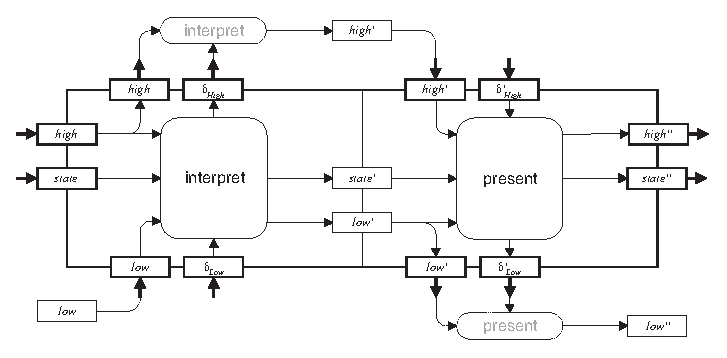
\includegraphics[width=\columnwidth]{images/LayerDataFlow}
\caption{Data flow in a Proxima layer.} \label{proximaDataFlow}
\end{figure}


The Proxima editor uses the described combinators for the description of its architecture.
Although the precise data flow of a Proxima layer is beyond the scope of this paper, we show a general overview in Figure~\ref{proximaDataFlow}. The main differences are that instead of mapping one data level onto another, a Proxima layer maps {\em edit operations} on a data level onto edit operations on the other level. Hence, each layer must also keep track of the actual data at each level. The edit operations are the deltas in the figure, whereas the data levels are the {\em high} and {\em low} values, which are threaded through the layer and switch between being vertical and horizontal parameters. 


The data flow in the figure is encoded in the type definition for a Proxima layer. For the edit operations (the $\delta$'s in Figure~\ref{proximaDataFlow}), we use distinct types for edit operations going up (\p{editH} and \p{editL}) and edit operations going down (\p{editH'} and \p{editL'}). The reason for this distinction is that upward edit operations are often of a different nature than the downward ones. The code below is actual Proxima source code:

\begin{small}
\begin{verbatim}
data Layer m state high low editH editL editH' editL' =
       Layer { interpret :: LayerFn m (state, high) (low,  editL)
                                      (state, low)  (high, editH)
             , present   :: LayerFn m (state, low)  (high, editH')
                                      (state, high) (low,  editL')
             }
\end{verbatim}
\end{small}


\section{Conclusions and future work} \label{sect:conclusions}

The combinators presented in this paper make it possible to specify layered editor architectures in a concise and transparent way. With a small number of definitions, a layered architecture can be described, clearly showing the data flow between the layers. The combinators have been heap profiled to ensure that no memory leaks are present, and have been used to implement the Proxima prototype as well as a database web-interface system.

Because the architecture description language is embedded in the implementation language, the architecture of a system forms part of the implementation of the system. We do not need to translate the architecture to an implementation, and hence, the implementation is guaranteed to comply with the architecture and vice versa.

We have shown that we can use Haskell to describe the various aspects of an ADL; \p{lift} and \p{combine} are the connectors; and the applications of \p{lift} and \p{combine} determine the configuration and the protocols at the connection points.

In the paper we have assumed that once we call a (combined) step function, the information flows through all the layers. In a real editor this might not always be the case; if the user adds some extra white-space this might be recorded in the state at one of the intermediate levels, upon which the presentation process can be resumed. We can also envision a situation where information flows up and down a few times between two adjacent layers, until a situation is reached in which a change has to be propagated to yet another layer. Note that we actually only require that the {\em upper protocol of a lower layer corresponds to the lower protocol of its upper layer}. 

We foresee however that we might use the type system to describe much more complicated protocols. An open question, and a matter of debate, is whether this should be done by exploiting the Haskell type system further, or whether one should move to more expressive type systems such as found in Agda \cite{norell:thesis}. Only experimenting and comparing solutions can give a definitive answer. Another area of research concerns how dynamic aspects of the architecture, such as invariants and constraints on the data, can be described and, if possible, verified.

The combinator language in this paper has been tailored to a specific kind of architectures: those of layered editors. Although we use the term editor in a broad sense, also including spreadsheets, e-mail agents, etc., further research should explore the possibilities of using Haskell to describe other kinds of architectures. For us the experiment to model the structure of the system using Haskell has been a successful experience, and we hope that this paper will inspire others to pursue the approach for different classes of architectures.  

%%%%%%%%%%%%%%%%%%%%%%%%%%%%%%%%%%%%%%%%%%%%%%%%%%%%
%%%%%%%%%%%%%%%%%%%%%%%%%%%%%%%%%%%%%%%%%%%%%%%%%%%%
\bibliographystyle{plainnat}
\bibliography{../proxima}
\end{document}

